\chapter{Conclusion}
brief of conclusion

\section{Conclusion of Problems}
Tell about solving the problem

\section{Conclusion of Method}
Tell about solving using method

\section{Conclusion of Experiment}
Tell about solving in the experiment

\section{Conclusion of Result}
tell about result for purpose of this research.

\section{Aip Suprapto Munari/1164063}
\subsection{Teori}
\begin{enumerate}

\item Mengapa Kata-Kata Harus di Vektorisasi
\par Kata harus divektorisasi karena mesin hanya mampu membaca data dalam tipe/bentuk angka. Oleh sebab itu, diperlukannya vektorisasi kata untuk mampu mebaca data tersebut. 
\par
\begin{itemize}
\item Gambar :
\par Penjelasan : Berdasarkan pengertian diatas, ada beberapa contoh yang bisa diterapkan. Untuk salah satu contoh dari klasifikasi data sendiri dapat diliat pada gambar berikut \ref{vektorisasikata}.
\begin{figure}
\centering
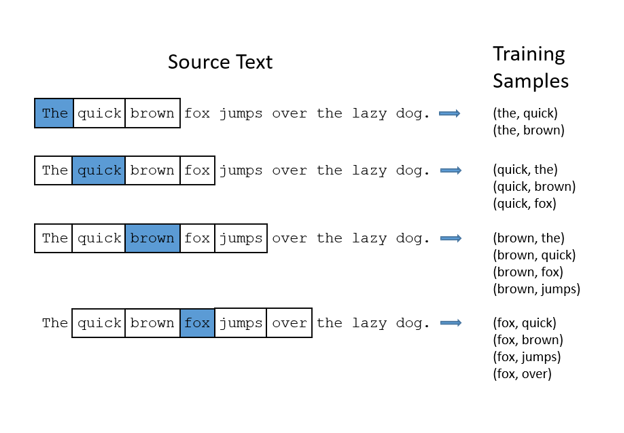
\includegraphics[scale=0.6]{figures/AIP/d1.PNG}
\caption{Vektorisasi Kata Aip}
\label{text-Aip}
\end{figure}
\end{itemize}

\item Mengapa Dimensi Dari Vektor Dataset Google Bisa Sampai 300
\par Setiap nilai dalam vektor 300 dimensi yang terkait dalam sebuah kata "dioptimalkan" dalam  beberapa hal untuk menangkap aspek yang  berbeda. Dengan kata lain masing-masing dari 300 nilai sesuai dengan beberapa fitur abstrak kata. Menghapus kombinasi nilai-nilai ini secara acak akan menghasilkan vektor yang mungkin kurang informasi penting tentang kata tersebut dan mungkin tidak lagi berfungsi sebagai representasi yang baik dari kata itu. Atau singkat cerita mungkin ada lebih dari 3 miliar kata-kata dan kalimat atau data yang tidak mungkin disimpan dalam 1 dimensi vektor maka disimpan menjadi 300 dimensi vektor untuk mengurangi kegagalan memori.
\par
\begin{itemize}
\item Gambar :
\par Penjelasan : Berdasarkan pengertian diatas, ada beberapa contoh yang bisa diterapkan. Untuk salah satu contoh dari klasifikasi data sendiri dapat diliat pada gambar berikut \ref{googleDataset}.
\begin{figure}
\centering
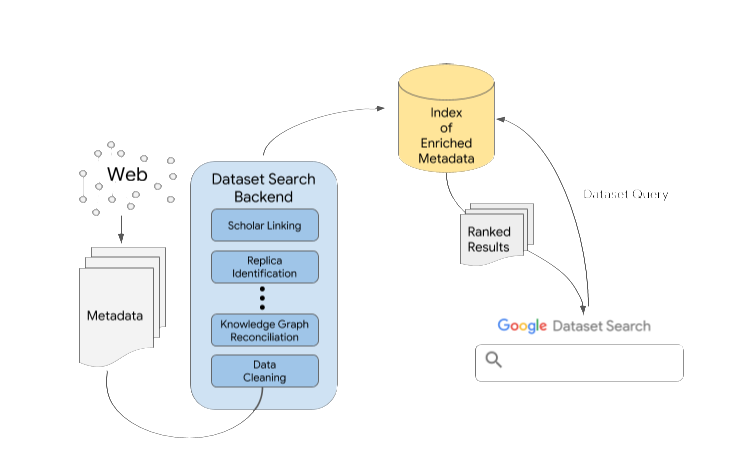
\includegraphics[scale=0.16]{figures/AIP/d2.PNG}
\caption{Google Dataset Aip}
\label{text-Aip}
\end{figure}
\end{itemize}

\item Konsep Vektorisasi Kata 
\par Konsep vektorisasi data merupakan kata-kata yang di inputkan pada mesin learning. Dan outputan nya berupa kara-kata atau keyword dari pencarian yang telah di lakukan sebelumnya. Contoh nya pada saat kita melakukan pencarian di youtube maupun pencarian google. Maka akan muncul hasil dari pencarian dari kata-kata yang telah kita cari atau input.
\par
\begin{itemize}
\item Gambar :
\par Penjelasan : Berdasarkan pengertian diatas, ada beberapa contoh yang bisa diterapkan. Untuk salah satu contoh dari klasifikasi data sendiri dapat diliat pada gambar berikut \ref{vekktorisasikata}.
\begin{figure}
\centering
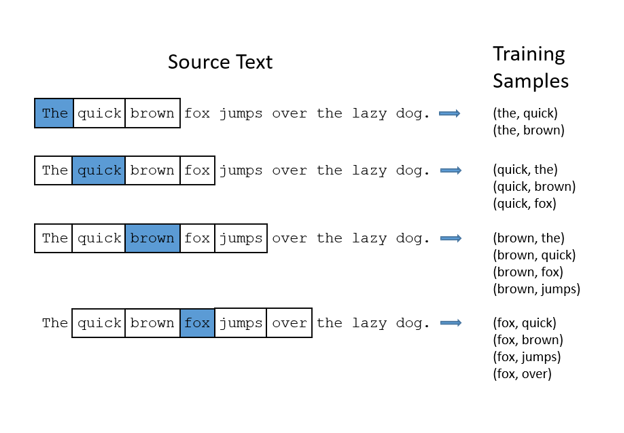
\includegraphics[scale=0.3]{figures/AIP/d1.PNG}
\caption{Vektorisasi Kata Aip}
\label{text-Aip}
\end{figure}
\end{itemize}

\item Konsep Vektorisasi Dokumen 
\par Konsep vektorisasi dokumen yaitu mesin akan membaca terlebih dahulu semua kalimat yang berada pada dalam dokumen dan nanti kalimat tersebut akan di pecah menjadi kata-kata.
\par
\begin{itemize}
\item Gambar :
\par Penjelasan : Berdasarkan pengertian diatas, ada beberapa contoh yang bisa diterapkan. Untuk salah satu contoh dari klasifikasi data sendiri dapat diliat pada gambar berikut \ref{vektorisasidokumen}.
\begin{figure}
\centering
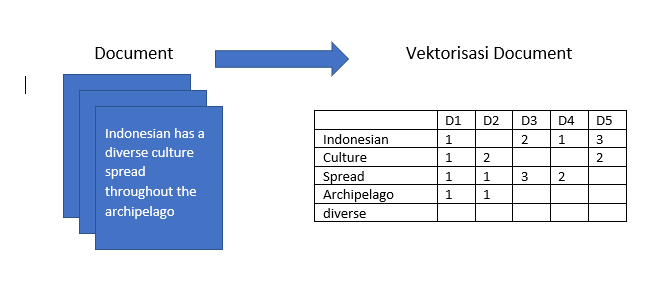
\includegraphics[scale=0.3]{figures/AIP/d3.PNG}
\caption{Vektorisasi Dokumen Aip}
\label{text-Aip}
\end{figure}
\end{itemize}

\item Mean dan Standar Deviasi
\par Mean adalah teknik penjelasan kelompok yang didasarkan atas nilai rata-rata dari kelompok tersebut. Rata-Rata (mean) ini didapat dengan menjumlahkan data seluruh individu dalam kelompok itu, kemudian dibagi dengan jumlah individu yang ada pada kelompok tersebut. Standar deviasi adalah nilai statistik yang digunakan untuk menentukan bagaimana sebaran data dalam sampel, dan seberapa dekat titik data individu ke mean atau rata-rata nilai sampel.Sebuah standar deviasi dari kumpulan data sama dengan nol menunjukkan bahwa semua nilai-nilai dalam himpunan tersebut adalah sama. Sebuah nilai deviasi yang lebih besar akan memberikan makna bahwa titik data individu jauh dari nilai rata-rata.
\par
\begin{itemize}
\item Gambar :
\par Penjelasan : Berdasarkan pengertian diatas, ada beberapa contoh yang bisa diterapkan. Untuk salah satu contoh dari klasifikasi data sendiri dapat diliat pada gambar berikut \ref{mean dan Standar Deviasi}.
\begin{figure}
\centering
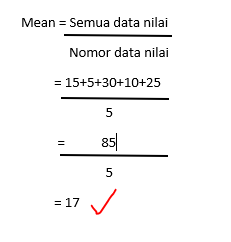
\includegraphics[scale=0.2]{figures/AIP/d4.PNG}
\caption{Mean Aip}
\label{text-Aip}
\end{figure}
\begin{figure}
\centering
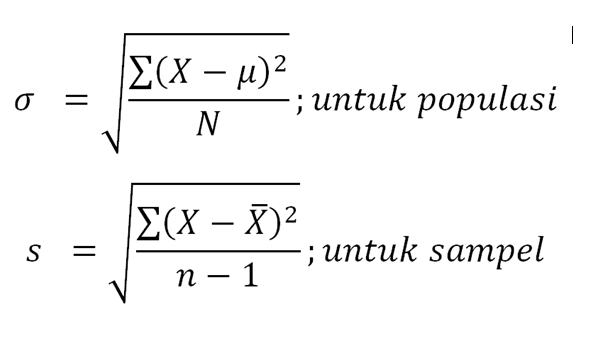
\includegraphics[scale=0.2]{figures/AIP/d5.PNG}
\caption{Standar Deviasi Aip}
\label{text-Aip}
\end{figure}
\par
\end{itemize}

\item Skip Gram
\par Skip-Gram mencoba memprediksi vektor kata-kata yang ada di konteks diberikan vektor kata tertentu. Skip-gram membuat sepasang kata target dan konteks sebagai sebuah instance.
\par
\begin{itemize}
\item Gambar :
\par Penjelasan : Berdasarkan pengertian diatas, ada beberapa contoh yang bisa diterapkan. Untuk salah satu contoh dari klasifikasi data sendiri dapat diliat pada gambar berikut \ref{skipgram}.
\begin{figure}
\centering
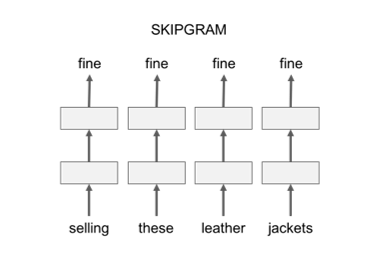
\includegraphics[scale=0.2]{figures/AIP/d6.PNG}
\caption{Skip-Gram Aip}
\label{text-Aip}
\end{figure}
\end{itemize}
\end{enumerate}

